
\interfootnotelinepenalty=10000
\usepackage[USenglish]{babel} %francais, polish, spanish, ...
\usepackage[T1]{fontenc}
%\usepackage[ansinew]{inputenc}
\usepackage{color}
\usepackage{mathtools}
%\usepackage{hyperref}
%\usepackage{subfig}


\usepackage{lmodern} %Type1-font for non-english texts and characters
\usepackage{algorithm}
\usepackage[noend]{algpseudocode}
\usepackage{mnsymbol}

%% Packages for Graphics & Figures %%%%%%%%%%%%%%%%%%%%%%%%%%
\usepackage{graphicx} %%For loading graphic files
\usepackage{amsmath}
\usepackage{amsthm} 
\usepackage{thmtools}
\usepackage{amsfonts}
\usepackage[all,cmtip]{xy}
\usepackage{tikz}


%\declaretheorem{Lemma}
%\declaretheorem{prop}

%\DeclareMathOperator{\sign}{sgn}
%\DeclareMathOperator{\coef}{coef}
%\DeclareMathOperator{\var}{var}
%\DeclareMathOperator{\eqs}{eqs}
%\DeclareMathOperator{\feas}{feas}
%\DeclareMathOperator{\UB}{UB}
%\DeclareMathOperator{\lb}{lb}
%\DeclareMathOperator{\FMcomb}{FM-comb}
%\DeclareMathOperator{\Gcomb}{Gauss-comb}
%\DeclareMathOperator{\proj}{proj}
%\DeclareMathOperator{\Pos}{Pos}
%\DeclareMathOperator{\Neg}{Neg}
%\DeclareMathOperator{\rhs}{rhs}
\newcommand{\sign}{\mathit{sgn}}
\newcommand{\coef}{\mathit{co}}
\newcommand{\var}{\mathit{var}}
\newcommand{\VAR}{\mathit{VAR}}
\newcommand{\eqs}{\mathit{eqs}}
\newcommand{\feas}{\mathit{feas}}
\newcommand{\UB}{\mathit{UB}}
\newcommand{\UBc}{\mathit{UBineq}}
\newcommand{\lb}{\mathit{lb}}
\newcommand{\lbc}{\mathit{lbineq}}
\newcommand{\FMcomb}{\mathit{FM}}
\newcommand{\Gcomb}{\mathit{GA}}
\newcommand{\proj}{\mathit{proj}}
\newcommand{\Pos}{\mathit{Pos}}
\newcommand{\Neg}{\mathit{Neg}}
\newcommand{\rhs}{\mathit{rhs}}
\newcommand{\bounds}{\mathit{bounds}}
\newcommand{\ie}{\mathcal{IE}}
\newcommand{\xx}{\mathcal{X}}
\newcommand{\vea}{\mathbf{co}}
\newcommand{\ttt}{\texttt{t}}
\newcommand{\trt}[1]{\texttt{#1}}
\newcommand{\mi}{\mathit}

\newcommand{\false}{\texttt{false}}
\newcommand{\true}{\texttt{true}}
\newcommand{\nul}{\texttt{null}}
\newcommand{\ve}{\mathbf}
%\newcommand\lhs[1]{\text{lhs}(#1)}
%\newcommand\rhs[1]{\text{rhs}(#1)}
%\newcommand\coef[1]{\text{coef}(#1)}
%\newcommand\LB[1]{\text{LB}_{#1}}
%\newcommand\UB[1]{\text{UB}_{#1}}
\newcommand{\lig}[4]{\ve{#1}\cdot\ve{#2}#3#4}
\newcommand\red[1]{\textcolor{red}{#1}}
\newcommand\blue[1]{\textcolor{blue}{#1}}
\newcommand{\set}[2]{\{\;{#1}\;|\;{#2}\;\}}
\newcommand{\odef}{\overset{\text{def.}}=}
\newcommand{\mc}{\mathcal}
\algdef{SE}[DOWHILE]{Do}{doWhile}{\algorithmicdo}[1]{\algorithmicwhile\ #1}%
\newcommand{\argmin}{\operatornamewithlimits{argmin}}
\newcommand{\StateInd}{\State\hspace{\algorithmicindent}}
\newcommand{\pr}{\mathit{PR}}
\newcommand{\prs}{\mathit{PRS}}
\newcommand{\ens}{\Leftrightarrow}

%\algdef{SE}[DOPAR]{DoPar}{doParWhile}{\algorithmicdo\textbf{ in parallel for\ }}[1]{\algorithmicwhile\ #1}%
\algdef{SE}[DOPAR]{DoPar}{doParUntil}{\algorithmicdo\textbf{ in parallel for\ }}[1]{\algorithmicuntil\ #1}%

\algdef{SE}[SUBALG]{Indent}{EndIndent}{}{\algorithmicend\ }%
\algtext*{Indent}
\algtext*{EndIndent}

\newtheorem{prop}{Proposition}
\newtheorem{lemma}{Lemma}
\newtheorem{cor}{Corollary}

\newcounter{para}
%\newcommand\mypara[1]{\par\refstepcounter{para}\textbf{\thep‌​ara\space#1\space}}
\newcommand\mypara[1]{\newline\par\refstepcounter{para}\textbf{\thepara}\space \textbf{#1} \space}
%\newcommand\mypara{\par\refstepcounter{para}\thepara\space}
%\usepackage[thmmarks,...]{ntheorem}
\newcommand{\Sec}{F}
\newcommand{\Ca}{\mi{Cap}}
\newcommand{\Vol}{\mi{V}}
\newcommand{\Weight}{\mi{W}}
\newcommand{\weight}{\mi{w}}
\newcommand{\BonjeanStations}{\mi{BS}}
\newcommand{\bonjean}{bf}
\newcommand{\Bonj}{B}
\newcommand{\shear}{\mi{sf}}
\newcommand{\Prop}{P}

\theoremstyle{definition}
%\newtheorem{example}{Example}[section]
\newtheorem*{theorem}{Theorem}

\theoremstyle{definition}
\newtheorem{examplex}{Example}[section]
\newenvironment{example}
  {\pushQED{\qed}\renewcommand{\qedsymbol}{$\triangle$}\examplex}
  {\popQED\endexamplex}
	
%\newtheoremstyle{named}{}{}{\itshape}{}{\bfseries}{.}{.5em}{\thmnote{#3}}
%\theoremstyle{named}
%\newtheorem*{namedtheorem}{Theorem}

\begin{document}
%\section*{In short}
%The network of a liner shipping company consists of several services, which each connects different ports in a given route. These services are usually circular, i.e. a vessel sailing on a service will later on return to the port of origin from where it will sail the same route. In between a vessel's return to its port of origin, other vessels sail on the same route such that the service is repeated at a given offset such as a week. The schedule of the vessels between two points in time can be illustrated in a time-space graph with the time (in days) along the $x$-axis and the ports along the $y$-axis. An example of services and a corresponding time-space graph can be seen in Figure \ref{fig:time-space}.
%
%%The task of the company is then either to transport specified cargo from given ports at given times to other ports before given points in time -- preferable in the best (cheapest)possible way -- or they need to decide which bookings they should take, i.e. to whom they should sell their transportation services, such that this is done and their profit is maximized.
 %
%The task of the company is to decide which bookings they should take, i.e. to whom they should sell their transportation services, of course in such a way that the cargo specified by these bookings are transported from the specified time and port to the destination time and port. Of course, it is in the interest of the company to do this in a way such that their profit is maximized, and the money earned on each container depends on properties such as the type of container (length, reefer/non-reefer-property, weight) as well as the combination of the port and day of origin and destination port and day. On the other hand, loading on unloading containers cost money, and depends on the port in which the (un)loading takes place. [Leaving at yard]
 %
%When solving this problem, we transform the mentioned time-space graph into a directed, multi-commodity flow graph, called the \emph{transshipment} graph, which is described further below. The idea is that at each port call, containers can stay on board the vessel or it can be unloaded to the yard, from where it is either picked up (because it is its final destination) or it stays until later. Likewise, containers from the yard can either be loaded onto the vessel or stay on the yard. These containers on the yard are either directly delivered there (because it is their port of origin) or it has been there since the last port call for the port in question.
%A time-space graph as described above is therefore expanded to the {transshipment} graph in the following way:
%For each port call $v=(t,p,s)$, where $s$ is a ship that calls port $p$ at time $t$ in the time-space graph, $6$ nodes are created, $n^v_{\texttt{si}}$, $n^v_\texttt{so}$, $n^v_\texttt{yi}$, $n^v_\texttt{yo}$, $n^v_{\texttt{on}}$, and $n^v_\texttt{off}$, and $6$ edges between those nodes, corresponding to the described possible actions at that port call are created, $e^v_\texttt{unld}$, $e^v_\texttt{ship}$, $e^v_\texttt{load}$, $e^v_\texttt{yard}$, $e^v_\texttt{on}$, and $e^v_\texttt{off}$; see Figure~\ref{fig:flownode}. 
%We further create edges  $(n^v_\texttt{so}, n^{v'}_\texttt{si})$ for all pairs $(v,v')$ of subsequent port calls in a route in the time-space graph (corresponding to the cargo being on board a sailing ship), and we make edges $(n^v_\texttt{yo}, n^{v'}_\texttt{yi})$ for all subsequent port calls relating to the same port (corresponding to containers being left at the yard until later). Finally, we create (further) explicit source-nodes to be able model what is on the vessels and yards, respectively, in the beginning of the time-space graph, and likewise we create sink-nodes to model what is on the vessels and yards, respectively at the end of the time-space graph. That is, for all ships $s$ we create nodes $n^s_\texttt{start},  n^s_\texttt{end}$ and edges $(n^s_\texttt{start}, n^v_\texttt{si}), (n^{v'}_\texttt{so}, n^s_\texttt{end})$, where $v$ is the first port call and $v'$ the last port call in $s$'s route (in the time-space-graph). Likewise, for all ports $p$, we create nodes $n^p_\texttt{start}, n^p_\texttt{end}$ and edges $(n^p_\texttt{start}, n^v_\texttt{yi}), (n^{v'}_\texttt{yo}, n^p_\texttt{end})$, where $v$ is the first port call relating to $p$ and $v'$ is the last port call relating to $p$.
%
%The sources are then $\set{n^v_\texttt{on}}{v \text{ is a port call in time-space graph}}\cup\set{n^s_{start}}{s\text{ is a ship}}\cup\set{n^p_{start}}{p\text{ is a port}}$, while the sinks are $\set{n^v_\texttt{off}}{v \text{ is a port call in time-space graph}}\cup\set{n^s_{end}}{s\text{ is a ship}}\cup\set{n^s_{end}}{p\text{ is a port}}$. [within a time treshold]. There is one commodity for each type of container $\tau \in T$ (see previously/later).
%
\section*{Transshipment graph}
$S$ is the set of ships that sails between ports in the set $P$.  
The port visits takes place between now (day $0$) and a given day $\mathbf{d}\in \mathbb{N}$; we let $D := \{0,1,\ldots, \mathbf{d}\}$ denote these day numbers.
%
Each ship $s\in S$ has a given route of ports that it visits in succession. This route is given by a sequence 
\[
r_s = ((p^s_1, d^s_1), (p^s_2, d^s_2), \ldots, (p^s_{l_s},d^s_{l_s}))\in (P\times D)^{l_s},
\]
where the $i$'th element in the sequence, $r_s(i) := (p^s_i, d^s_i)$, indicates the $i$'th port in the route and the day it is visited.
%
We then define the set of \emph{visitation nodes}, as $V := \bigcup_{s\in S}\set{r_s(i)}{0\leq i\leq l_s}$.

Given the routes of the ships, we can define the sequence of visitation nodes at a port $p\in P$ by ordering the set 
$W_p:= \bigcup_{s\in S}\bigcup_{1\leq i \leq l_s}\set{r_s(i)}{r_s(i)=(p,d)\text{ for a }d\in D}$ according to the day component\footnote{For simplicity, we assume that  $r_s(i) \neq r_{s'}(j)$ for any $s \neq s'$ and any $i,j$. Otherwise, each elements in $V$ are augmented with the ship $s$ that makes the port call, and an ordering on $S$ is assumed (and used for ordering $W_p$), too.}.
For $1\leq i\leq |W_p|$, we let $v_p(i)$ denote the $i$'th elements in this sequence, and we let $\textit{day}_p(i)$ denote the day-component of $v_p(i)$.  
\\
\\
Given the visitation nodes $V$, we now define the \emph{transshipment graph} $\mc{G}=(\mc{N},\mc{E})$ as follows.

For each $v\in V$ we create the following set of nodes, $\mc{N}_v:=\{n^v_{\texttt{si}}, n^v_\texttt{so}, n^v_\texttt{yi}, n^v_\texttt{yo}, n^v_{\texttt{on}}, n^v_\texttt{off}\}$.%\footnote{\texttt{si} stands for ``ship in'', \texttt{so} stands for ``ship out'', \texttt{yi} for ``yard in'', \texttt{yo} for ``yard out'', \texttt{on} for ``bookings on'', and \texttt{off} for ``bookings off''.}. 
%
We then  we create a set of edges, $\mc{E}_v = \{e^v_\texttt{unld}, e^v_\texttt{ship}, e^v_\texttt{load}, e^v_\texttt{yard}, e^v_\texttt{on}, e^v_\texttt{off}\}$, where
\begin{align*}
e^v_\texttt{unld} &= (n^v_\texttt{si},n^v_\texttt{yo}),
& e^v_\texttt{ship} &= (n^v_\texttt{si},n^v_\texttt{so}),
& e^v_\texttt{load} &=(n^v_\texttt{yi},n^v_\texttt{so}),\\
 e^v_\texttt{yard} &=(n^v_\texttt{yi},n^v_\texttt{yo}),
& e^v_\texttt{on}   &=(n^v_\texttt{on},n^v_\texttt{yi}), \quad\text{ and }
& e^v_\texttt{off} & =(n^v_\texttt{yo},n^v_\texttt{off});
\end{align*}
see Figure \ref{fig:nodesAndEdges}. % \footnote{\texttt{unld} stands for ``unload from ship'', \texttt{ship} for ``stay on ship'', \texttt{load} for ``load from yard'', \texttt{yard} for ``stay on yard'', \texttt{on} for ``loading bookings on'', and \texttt{off} for ``taking bookings off''.}. 
%
\begin{figure}[htbp]
	\centering
		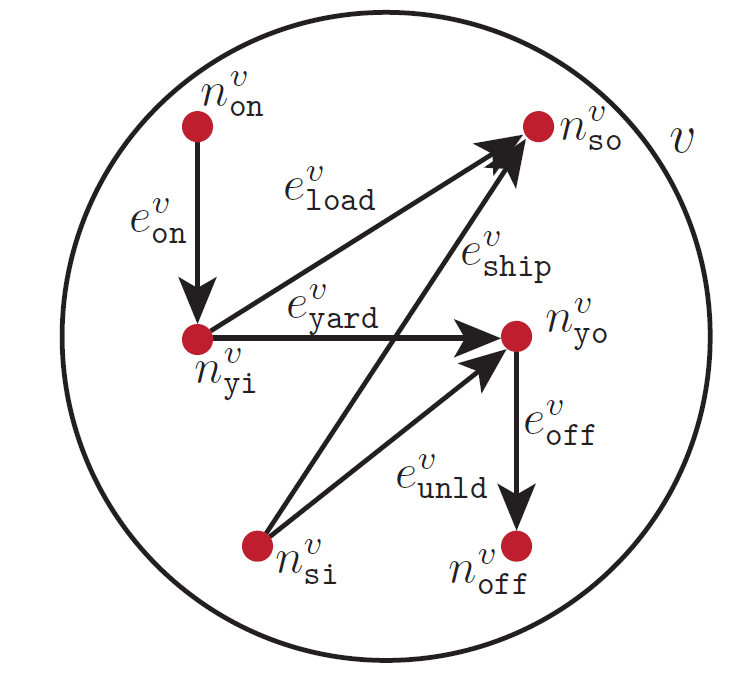
\includegraphics{//fs4.itu.local/redirection/ajspur/Pictures/nodesandedgesforn.pdf}
	\caption{The nodes $\mc{N}_v$ and edges $\mc{E}_v$ created for the visitation node $v\in V$.}
	\label{fig:nodesAndEdges}
\end{figure}
The idea is, that $n^v_\texttt{si}$ denotes the ship (giving rise to the visitation node $v=(p,d)$) when it arrives at port $p$ at day $d$ (``$\texttt{si}$'' stands for ``ship in''), while $n^v_\texttt{so}$ denotes the ship when it leaves (``$\texttt{so}$'' stands for ``ship out''). $n^v_\texttt{yi}$ denotes the yard at the port just prior to the ship's arrival, while $n^v_\texttt{yo}$ denotes the yard at the ship's departure. From the yard, containers can be loaded to the ship, corresponding to the edge $e^v_\texttt{load}$, or it can stay on the yard, corresponding to $e^v_\texttt{yard}$. From the ship, containers can be unloaded ($e^v_\texttt{unld}$), or they can stay on the ship ($e^v_\texttt{ship}$). Finally, containers stemming from bookings can be introduced to the yard from ``outside'' just prior to the ships arrival ($e^v_\texttt{on}$), while others can be removed from the yard when the ships departure ($e^v_\texttt{off}$). 


To model the routes of the ships, we firstly create a distinguished ``start node'', $n^s_{\texttt{start}}$ and a distinguished ``end node'', $n^s_{\texttt{end}}$ for each $s \in S$, and we create edges $e^s_{0} = (n^s_{\texttt{start}}, n^{r_s(1)}_\texttt{si})$ and $e^s_{l_s} = (n^{r_s(l_s)}_\texttt{so}, n^s_{\texttt{end}})$. We then ``connect'' the route by creating edges $e^s_i= (n^{r_s(i)}_\texttt{so}, n^{r_s(i+1)}_\texttt{si})$ for each $1\leq i < l_s$; see Figure~\ref{fig:routeEdges}. 
We let $\mc{E}_{\texttt{route}} = \bigcup_{s\in S}\set{e^s_i}{0\leq i \leq l_s}$. 

\begin{figure}[htbp]
	\centering
		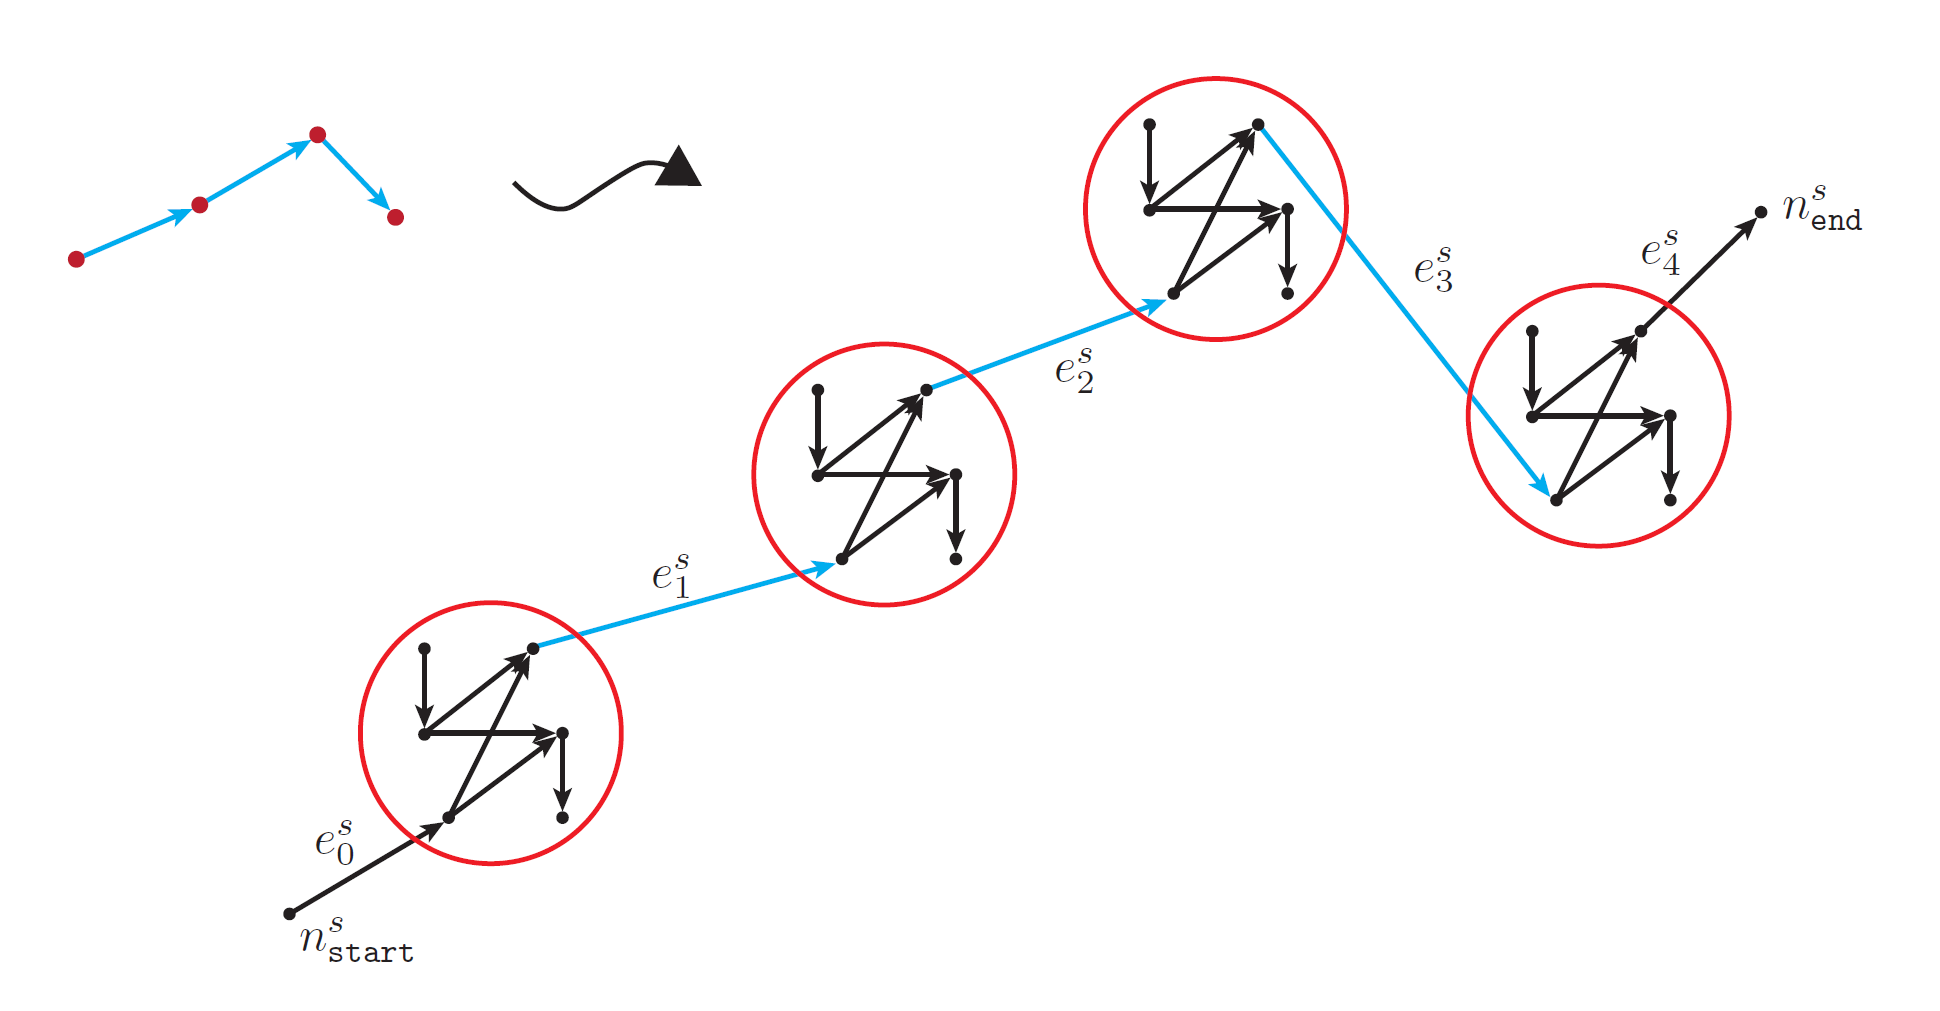
\includegraphics{//fs4.itu.local/redirection/ajspur/Pictures/routeEdges.pdf}
	\caption{Assuming that $s$'s entire route consists of four visitation nodes as depicted in the top left corner, then the corresponding nodes and edges in $\mc{G}$ made from this route are depicted in the rest of the figure. 
	}
	\label{fig:routeEdges}
\end{figure}

To model the possibility of transshipments, we similarly create a node $n^p_{\texttt{start}}$ and a node $n^p_{\texttt{end}}$ for all $p\in P$.  
We define $e^p_0 = (n^p_{\texttt{start}}, n^{v_p(1)}_\texttt{yi})$ and $e^p_{|W_p|} = (n^{v_p(|W_p|)}_\texttt{yo}, n^p_{\texttt{end}})$, and we further define $e^p_i := (n^{v_p(i)}_\texttt{yo}, n^{v_p(i+1)}_\texttt{yi})$ for each $1\leq i < |W_p|$. 

These constitute all the nodes and edges in $\mc{G}$, i.e.  
\begin{align*}
\mc{N} &= \bigcup_{v\in V}\mc{N}_{v}\;\dot\cup\bigcup_{s\in S}\{n^s_{\texttt{start}}, n^s_{\texttt{end}}\}\;\dot\cup\bigcup_{p\in P}\{n^p_{\texttt{start}}, 
n^p_{\texttt{end}}\}, \text{ and}\\
\mc{E} &= \bigcup_{v\in V}\mc{E}_{v}\;\dot\cup\;\mc{E}_{\texttt{route}}\;\dot\cup\bigcup_{p\in P}\set{e^p_i}{0\leq i \leq |W_p|}.
\end{align*}
\section*{Model}
\paragraph{Parameters}$\;$\\
%The ships described above transport containers on their routes, and these containers are divided into different types depending on eg. their length, weight and whether they are reefer containers or not. The type of a container is a very important factor for determining the revenue of transporting it from its origin to its destination, and bookings are also described partly in terms of these types. 
%
%Below we list some constants used for calculating the costs and revenue, respectively, for transporting containers of a given type from a given visitation node to another. Likewise we have a constant describing the given possible bookings that can be taken, plus what is on the various ships and ports at the starting point.\\\\
%
%Finally we will, for each ship, have some constraints describing the dependencies between the (number of) different types of containers on the ship in order for it to comply with e.g. capacity constraints and seaworthiness. This could be something as basic as a given capacity for each container type. We therefore have the following:

\begin{tabular}{lp{9,5cm}}
$\Gamma$&Set of types of containers\\
$\Gamma_{20}, \Gamma_{40}, \Gamma_{\texttt{R}}\subseteq \Gamma$&Set of container types with length $20'$, length $40'$, and that are reefers, respectively.\\
$C^{\tau,p}_{\texttt{M}} \in \mathbb{R}$&The cost of moving (loading or unloading) a container of type $\tau\in \Gamma$ in port $p\in P$.\\
$C^{\tau,p}_{\texttt{L}} \in \mathbb{R}$&The cost per day of having a container of type $\tau\in\Gamma$ lying at port $p\in P$.\\
$R^{\tau,p,p'}\in \mathbb{R}$&The revenue for transporting a container of type $\tau\in \Gamma$ from port $p\in P$ to port $p'\in P$.\\
$CN$&Set of constraints on the relationship between the number of each type of containers in a feasible stowing. Each $c\in C$ is a function $c:\Gamma\cup \{\texttt{rhs}\}\to\mathbb{R}$, where $c(\tau)$ is the coefficient for containers of the type $\tau$, and $c(\texttt{rhs})$ is the right-hand-side of the less-or-equal-to constraint (see later). 
\end{tabular}
\paragraph{Variables}
The decision variables are 
\[
x^{\tau,v}_e \in \mathbb{R}^+\quad \text{ for all } \tau\in \Gamma, v\in V, e\in \mc{E}.
\]
This denotes the number of containers of type $\tau$ that should be transported to port $p$ at time $d$ that ``flows'' on the edge $e$.

Likewise we define the auxiliary variables 
\[
w^{\tau}_e = \sum_{v\in V}x^{\tau,v}_e \in \mathbb{R}^+ \quad \text{ for all } \tau\in \Gamma, e\in \mc{E}_{\texttt{route}}. 
\]
For a $c\in CN$, $c(\tau)$ corresponds to the coefficient of the variable $w^\tau_e$ for any edge $e$ in the transshipment graph where cargo is transported on a ship, i.e. $\mc{E}_{\texttt{route}}$.
%
\paragraph{Objective function}
Income is made on all booking that are taken (all containers stowed on any of the ships), while there is a cost associated with loading and unloading containers (including transshipments), and for having the containers standing at the yard. Thus, the following is maximized [NB: where $D'<\frac{\mathbf{d}}{2}$ is a given deadline not previously described]:
\begin{align*}
&\sum_{\tau\in\Gamma}\sum_{(p',d') \in V}\Big(\sum_{(p,d) \in V. p<D'}x^{\tau,(p',d')}_{e^{(p,d)}_{\texttt{on}}}\cdot R^{\tau,p,p'}
+ \sum_{s \in S} x^{\tau,(p',d')}_{e^{s}_{0}}\cdot R^{\tau,p^s_1,p'} 
+ \sum_{p \in P}x^{\tau,(p',d')}_{e^{p}_{0}}\cdot R^{\tau,p,p'}\Big)\\
%
&-\sum_{(p,d) \in V}\sum_{\tau\in\Gamma}\sum_{v' \in V}\big(x^{\tau,v'}_{e^{(p,d)}_{\texttt{load}}} + x^{\tau,v'}_{e^{(p,d)}_{\texttt{unld}}}\big)\cdot C^{\tau,p}_{\texttt{M}}\\
&-\sum_{p \in P}\sum_{i =1}^{|W_p|-1}\sum_{\tau\in\Gamma}\sum_{v' \in V}x^{\tau,v'}_{e^{v_p(i)}_{\texttt{nxP}}}\cdot(\mathit{day}_p(i+1)-\mathit{day}_p(i))\cdot C^{\tau,p}_{\texttt{L}}\\
%&-\sum_{p \in P}\sum_{\tau\in\Gamma}\sum_{v' \in V}\big(x^{\tau,v'}_{e^{p}_{0}}\cdot ?_3 + x^{\tau,v'}_{e^{p}_{|W_p|}}\cdot ?_4\big)\cdot C^{\tau,p}_{\texttt{L}} )\\
\end{align*}
%\red{Comment: $?_1$ is because we don't know where the cargo on each ship when arriving comes from (has been set to $p^s_1$), $?_2$ is because we don't know where the cargo at the yard of each port comes from (has been set to $p$ itself),
%$?_3$ is because we don't know how long the cargo at each yard has been lying there (but we could just set it to $\mathit{day}_p(1)$ (OBS: currently, we make it 0, I think)), $?_4$ is because we don't know how long the last cargo will be lying around (but we can just set it to $(\mathbf{d}-\mathit{day}_p(|W_p|))$ - there probably won't be anything anyway. Currently: it is set to 0). }

%\red{Comment: we should probably already have something on board (and not make that a variable, or, alternatively, fix the value. Also to avoid that the ship is just filled with stuff going to the first visitation node $v$ on the route to make easy profit). }
\paragraph{Constraints}$\;$\\
\textit{Flow conservation} 
At all internal nodes in the transshipment graph, the flow of containers of each type and destination should be preserved. I.e. for nodes with both ingoing and outgoing edges,  the incoming flow of containers (of a specific type and a specific destination-node) should equal the outgoing flow of containers (of that type and destination-node). That is, 
\[
\forall {n}\in \bigcup_{v\in V}\{n^v_{\texttt{si}}, n^v_\texttt{so}, n^v_\texttt{yi}, n^v_\texttt{yo}\}\; \forall \tau \in \Gamma\; \forall v \in V: 
\quad \sum_{e\in \mathit{In}(n)}x^{\tau, v}_e = \sum_{e\in \mathit{Out}(n)}x^{\tau, v}_e,
\]
where $\mathit{In}(n) = \set{(n',n'')\in\mc{E}}{n'' = n}$, and $\mathit{Out}(n) = \set{(n'',n')\in \mc{E}}{n'' = n}$ for all ${n}\in \mc{N}$.
\\\\
\textit{Outflow}
%At a visitation node $v\in V$ we can only take off/unload containers that were shipped to that node:
%\[
%\forall v,v'\in V\;\forall \tau \in \Gamma.\;v'\neq v:\quad 
%x^{\tau,v'}_{e^{v}_\texttt{off}} = 0.
%\]
%
%At every visitation node we take away from the yard/port what were shipped to that port:
%\[
%\forall v\in V, \tau \in \Gamma:\quad 
%x^{\tau, v}_{e^{v}_\texttt{off}} = x^{\tau, v}_{e^v_\texttt{yard}}+x^{\tau, v}_{e^v_\texttt{unld}}
%\]
%\textit{Everything is delivered}
Every container taken on board a ship must be delivered (at the right destination):
\[
\forall v\in V\;\forall\tau\in\Gamma:\quad
x^{\tau,v}_{e^{v}_{\texttt{off}}} = \sum_{e\in \mathit{InE}}x^{\tau,v}_e,
\]
where $\mathit{InE} = \bigcup_{v\in V}\{e^v_{\texttt{on}}\}\cup\bigcup_{s\in S}\{e^s_{0}\}\cup\bigcup_{p\in P}\{e^p_{0}\}$. 

\textit{Capacity constraints}
\[
\forall c\in CN\;\forall e\in \mc{E}_{route}:\quad
        \sum_{\tau \in \Gamma} c(\tau)\cdot w^\tau_e \leq c(\texttt{rhs})
\]
\textit{Restriction on variables}
To help with preprocessing, we add the following (redundant) constraints saying that a container is not transported later then it shold be delivered:
\[
\forall (p,d) \in V\; \forall e\in\mc{E}_{(p,d)}\;\forall \tau\in\Gamma\;\forall(p',d')\in V\;.\; d'< d :\quad x^{\tau, (p',d')}_{e} = 0.
\]
\end{document}